\section{Planning in NLG} \label{sec:domains}

In this section, we present the two domains: first the sentence
generation domain, then the instruction giving domain.


\subsection{Sentence generation as planning}






\subsection{Planning in instruction giving}

The object of the GIVE Challenge (``Generating Instructions in Virtual
Environments''; Koller et al.\
\citeyear{alexander07:_shared_task_propos}) is to build an NLG system
which is able to give natural-language instructions which will guide a
human user in performing some task in a virtual environment.  A map of
an example world is shown in Fig.~\ref{fig:give-development-world};
instructions for the first steps could be ``turn left; press the
button; turn right and walk through the door;'' and so forth.  From an
NLG perspective, GIVE makes for an interesting challenge because it is
a theory-neutral task that exercises all components of an NLG system,
and emphasizes the study of communication in a (simulated) physical
environment.  It also has the advantage that the user and the NLG
system can be physically in different places, as long as the 3D client
and the NLG system are connected over a network.  This makes it
possible to evaluate GIVE NLG systems on a large scale over the
Internet.  The first GIVE evaluation will take place in late 2008;
currently seven research teams from five countries are working on
developing systems to participate in the challenge.

\begin{figure}
\centering
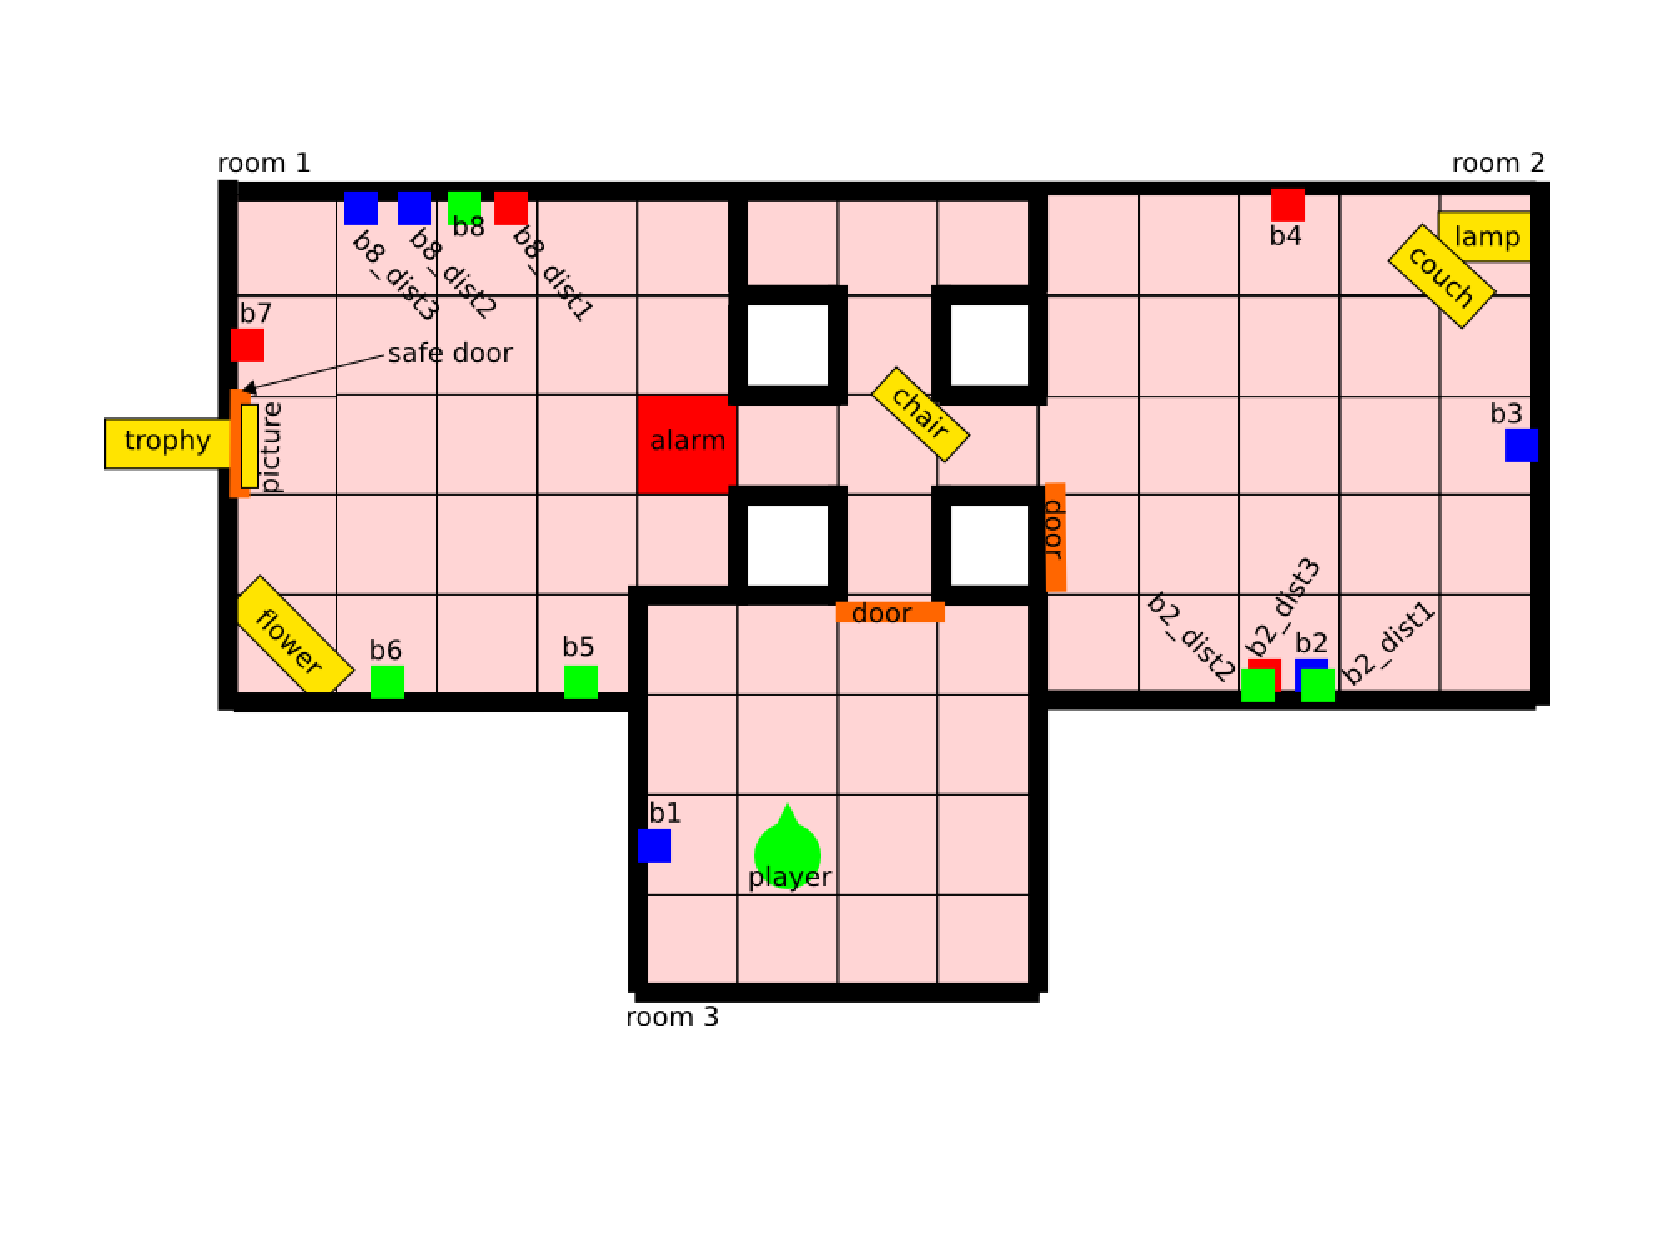
\includegraphics[width=1 \columnwidth]{give_world_no_expl}
\caption{Map of the GIVE development world.}
  \label{fig:give-development-world}
\end{figure}

\todo{explain world? -- yes, definitely}


One crucial component of a GIVE system is a planner which will compute
a domain plan that consists of the actions the user has to execute to
achieve the goal.  For these purposes, the virtual world is
discretized into a planning problem in which each object has a
symbolic position and orientation.  The first few action instances in
the example domain could be $turn-left(north,west)$, $move(pos-3-2,
pos-2-2, west)$, $manipulate-b_1-off-on(pos-2-2)$,
$turn-right(west,north)$, \todo{complete this} and so on.  Under the
current implementation of the planning problem, the shortest plan for
getting the player from the initial state to the goal (in which they
are holding the trophy) has 104 steps, most of which are ``move''
actions.  The bulk of the GIVE problem is therefore a variant of the
Gridworld problem, which also involves finding a route through a world
with discrete positions -- but with the need to press buttons in the
right order and with somewhat more complicated room shapes.

It is interesting to note that although the task of a GIVE NLG system
could be seen as mapping a domain plan to a sequence of NL
instructions, this mapping is not trivial.  It would be
\emph{possible} to express the last part of the above example plan as
``turn right; walk forward; walk forward; turn right; walk forward;
walk forward; turn left; walk forward'', but this is a very clumsy way
of phrasing the instruction ``turn around and walk through the door''
that will frustrate users and lead to bad evaluation results.  In
other words, it is important to aggregate multiple movement actions
into a single NL instruction.  On the other hand, it may be necessary
to generate instructions that don't correspond to domain actions.  For
instance, it will be necessary to find a correct referring expression
for $b_1$ in order to express the action
$manipulate-b_1-off-on(pos-2-2)$.  The interaction between referring
and instructing can go much deeper than that.  Imagine, for example,
that the user just entered the top right room, and we want to instruct
them to press $b_4$.  At that point in time, the user can see six
different buttons, and generating a single instruction of the form
``push X'' is difficult.  However, an instruction sequence like ``walk
forward; turn left; now press the button right in front of you'' will
be successful and natural.  Here the first two instructions do double
duty by preparing the simple referring expression ``the button right
in front of you'', which is only valid after the user's position and
orientation changed.  A generation system that is supposed to generate
such instruction sequences must be tightly integrated with the planner
in order to exploit the simultaneous effect of the first two
instructions on the world and on the communicative situation.

\todo{equivalent plans; plan recognition; real-time requirements}


%%% Local Variables: 
%%% mode: latex
%%% TeX-master: "experiences"
%%% End: 
